\chapter{Тестирование}\label{ch:ch3}

Реализованный model checker способен искать настоящие, нетривиальные ошибки в конкурентном коде. В этой главе мы продемонстрируем это утверждение на двух примерах: 

\section{LFAlloc}

Первый пример – это lock-free стек, выполняющий роль глобального кеша блоков в аллокаторе LFAlloc, который используется в алгоритме машинного обучения CatBoost и внутренних системах Яндекса \autocite{YaAlloc}. Реализация стека в ранней версии аллокатора содержала сложный сценарий ABA из нескольких десятков шагов. Уже после обнаружения ошибки для стека написали спецификацию на +Cal \autocite{YaSpec}, с помощью которой подтвердили наличие ошибки и верифицировали патч для нее.

Наш model checker находит тот же баг, но работает непосредственно с реализацией конкурентной структуры данных, а значит, не надо специфицировать стек на псевдокоде, расставлять метки атомарности, моделировать память и указатели.

%\iftoggleverb{pics}

\begin{figure}
	\centerfloat{
		\begin{tabular}{p{0.5\textwidth} p{0.5\textwidth}}
			\centering
			\vspace{0pt} \fbox{\parbox[t][.28\textheight]{0.48\textwidth}{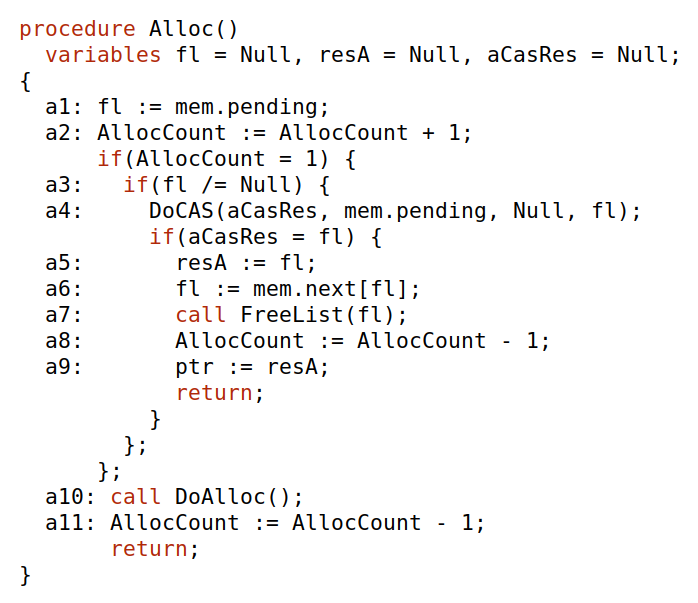
\includegraphics[width=0.48\textwidth]{specalloc}}}
			&
			\vspace{0pt} \fbox{\parbox[t][.28\textheight]{0.48\textwidth}{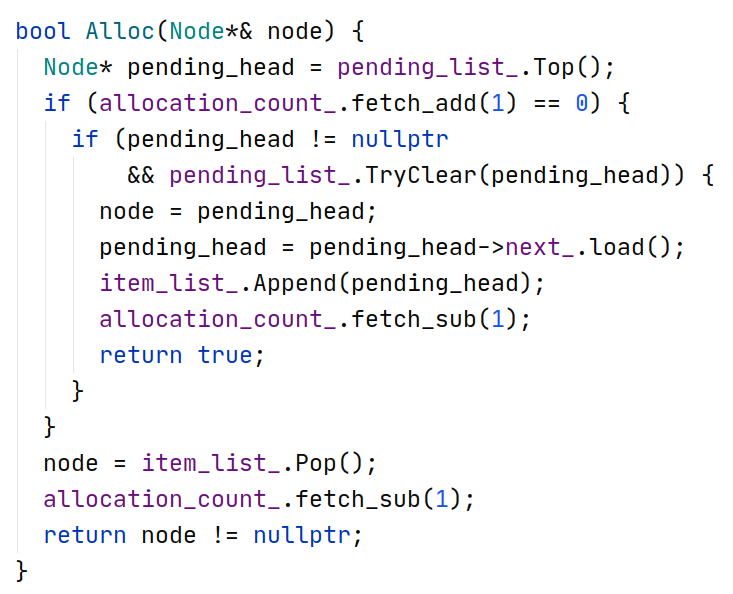
\includegraphics[width=0.48\textwidth]{checkeralloc}}}
			\\
			\hfil +Cal & \hfil \CC
		\end{tabular}
	}
	\bigskip
	\caption{Сравнение спецификации и кода на примере lock-free стека.}
\end{figure}

%\else
\begin{comment}

\begin{figure}
	\centerfloat{
		\begin{tabular}{p{0.5\textwidth} p{0.5\textwidth}}
			\centering
			
			\vspace{0pt}
			
			\fbox{\parbox[t][.28\textheight]{0.48\textwidth}{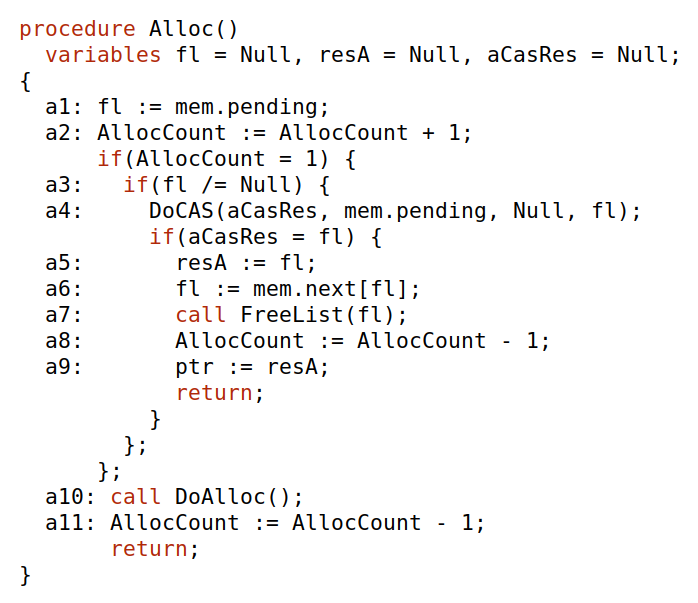
\includegraphics[width=0.48\textwidth]{specalloc}}}
			&
			\vspace{0pt} 
			
			\begin{minted}[fontsize=\tiny, frame=single, linenos=false]{c++}
 bool Alloc(Node*& node) {
	Node* pending_head = pending_list_.Top();
	if (allocation_count_.fetch_add(1) == 0) {
		if (pending_head != nullptr
		&& pending_list_.TryClear(pending_head)) {
			node = pending_head;
			pending_head = pending_head->next_.load();
			item_list_.Append(pending_head);
			allocation_count_.fetch_sub(1);
			return true;
		}
	}
	node = item_list_.Pop();
	allocation_count_.fetch_sub(1);
	return node != nullptr;
}
			\end{minted}
			
			
			\\
			\hfil +Cal & \hfil \CC
		\end{tabular}
	}
	\bigskip
	\caption{Сравнение спецификации и кода на примере lock-free стека.}
\end{figure}

%\fi
\end{comment}

При этом структуру теста можно не менять, а позаимствовать ее из спецификации на +Cal: поток в бесконечном цикле аллоцирует и деаллоцирует блоки памяти (узлы стека).

\begin{figure}
	\centerfloat{
		\begin{tabular}{p{0.5\textwidth} p{0.5\textwidth}}
			\centering
			\vspace{0pt} \fbox{\parbox[t][.2\textheight]{0.48\textwidth}{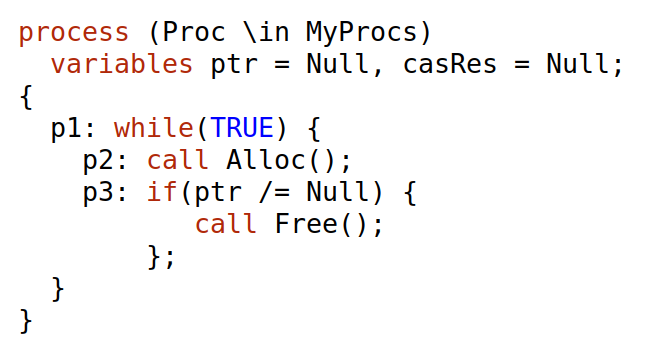
\includegraphics[width=0.48\textwidth]{spectest}}}
			&
			\vspace{0pt} \fbox{\parbox[t][.2\textheight]{0.48\textwidth}{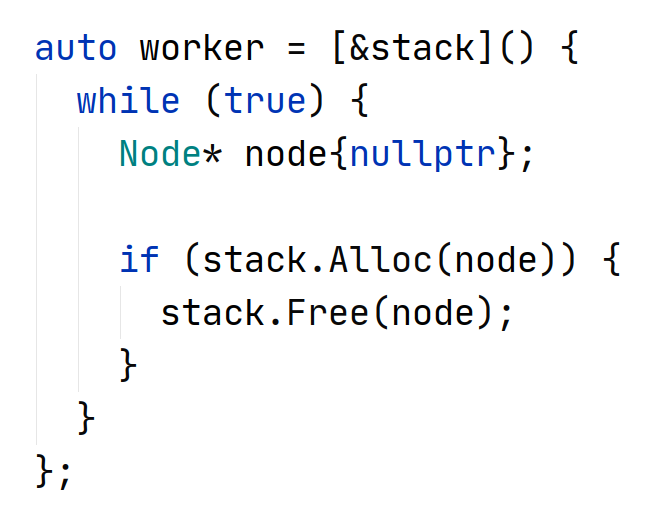
\includegraphics[width=0.38\textwidth]{checkertest}}}
			\\
			\hfil +Cal & \hfil \CC
		\end{tabular}
	}
	\bigskip
	\caption{Один и тот же тест для TLC и для model checker-а.}
\end{figure}

\begin{comment}

\begin{figure}
	\centerfloat{
		\begin{tabular}{p{0.5\textwidth} p{0.5\textwidth}}
			\centering
			\vspace{0pt} 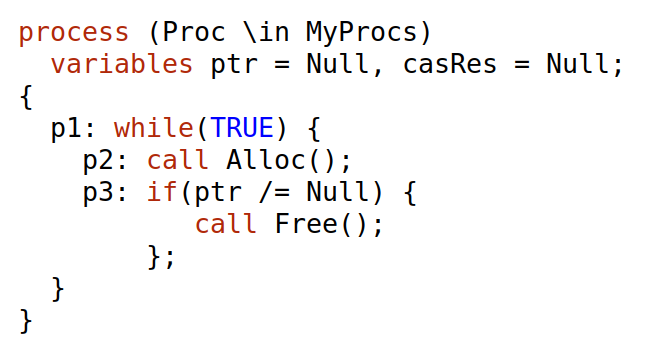
\includegraphics[width=0.5\textwidth]{spectest}
			&
			\vspace{0pt} 
			
			\begin{minted}{c++}
auto worker = [&stack]() {
	while (true) {
		Node* node{nullptr};

		if (stack.Alloc(node)) {
			stack.Free(node);
		}
	}
};
			\end{minted}
			
			\\
			\hfil +Cal & \hfil \CC
		\end{tabular}
	}
	\bigskip
	\caption{Один и тот же тест для TLC и для model checker-а.}
\end{figure}

\end{comment}

Реализация lock-free стека и тест для model checker-а приведены в приложении \ref{app:A}.

Траектория, напечатанная нашим model checker-ом (см. \ref{app:trace}), более читаема, чем траектория, которую печатает TLC: в ней для каждого шага печатается настоящий стектрейс и значения локальных переменных. По ней гораздо проще восстановить сценарий ABA.

Приведем статистику поиска данного бага model checker-ом и TLC:

%\begin{center}
\begin{table}
\centering
\begin{tabular}{| l | c | c |}
\hline
                   & model checker & TLC \\
                   \hline
 Длина траектории & 61 шаг & 76 шагов \\ 
 Найдено состояний & \numprint{17906188} & \numprint{26168885} \\  
 Найдено уникальных состояний & \numprint{4751588} & \numprint{7269203} \\
 Время                       & 29 cекунд & 8 минут\\
 	\hline
\end{tabular}

\bigskip
\captionsetup{justification=centering}
\caption{Статистика поиска ABA в LFAlloc.} 
\end{table}
%\end{center}

В четвертой главе будет описан инструмент model checker-а (недетерминизм, выражаемый в коде), который позволит сделать тест для стека более гибким – и, как следствие, сократить перебор и получить более короткую траекторию.

LFAlloc - пример со сложным (длинным) сценарием ABA. Следующий пример - про сложность другого рода: про поиск ошибки в большом коде.

\section{Executors}

Executors – фреймворк для асинхронного исполнения задач. Пользователю предоставляется сущность \emph{экзекьютора} (представленная интерфейсом \mintinline{c++}{IExecutor}) с единственной операцией – запланировать \emph{задачу} (произвольную функцию без аргументов и возвращаемого значения) для исполнения в некотором потоке.

Базовый экзекьютор – пул потоков фиксированного размера, разбирающих разделяемую очередь задач. Поверх этого пула можно писать декораторы, например, для последовательного исполнения задач или для поддержки приоритетов задач.

Код в таком фреймворке не похож на изолированную структуру данных: он гораздо больше и в нем много нетривильных конкурентных “деталей”: блокирующие и лок-фри очереди, спинлоки, вспомогательные примитивы синхронизации и т.п.

\iftoggleverb{pics}

\begin{figure}
	\centerfloat{
		\fbox{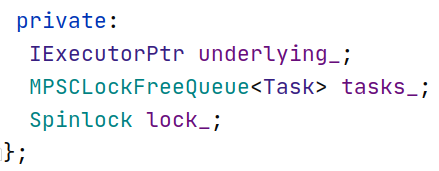
\includegraphics[scale=0.5]{strandfields}}
	}
	\bigskip
	\caption{Поля одного из экзекьюторов (Strand-а) – композиция конкурентных объектов.}\label{fig:strandfields}
\end{figure}

\else

\begin{listing}
	\centering
	
	\begin{minted}{c++}
    
class Strand : public IExecutor {
// implementation...

private:
	IExecutorPtr executor_;
	MPSCLockFreeQueue<Task> tasks_;
	Spinlock lock_;
};

	\end{minted}
	\caption{Поля одного из экзекьюторов (Strand-а) – композиция конкурентных объектов.}
	\label{strandfields}
\end{listing}

\fi

Рассмотрим \emph{Strand} (или \emph{Serial Executor}) – декоратор над пулом потоков, который исполняет все запланированные через него задачи в потоках декорируемого пула строго последовательно и в порядке их добавления.

В реализации этого декоратора легко допустить race condition при планировании / перепланировании служебной задачи, которая запускает пользовательские в потоках нижележащего пула. Такой race condition приведет к тому, что последняя пачка задач Strand-а может не выполниться.

\begin{figure}
	\centerfloat{
		\begin{tabular}{p{0.5\textwidth}p{0.5\textwidth}}
			\centering
			\vspace{0pt} \fbox{\parbox[t][.29\textheight]{0.48\textwidth}{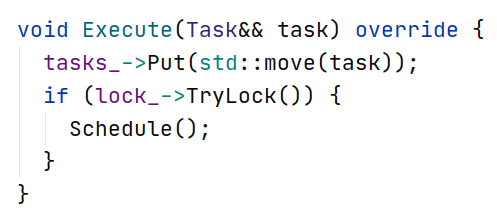
\includegraphics[width=0.48\textwidth]{exec}}}
			&
			\vspace{0pt} \fbox{\parbox[t][.29\textheight]{0.48\textwidth}{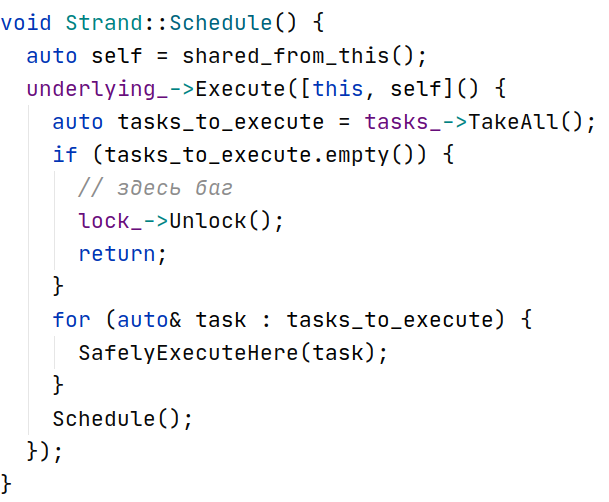
\includegraphics[width=0.48\textwidth]{sched}}}
		\end{tabular}
	}
	\bigskip
	\caption{Фрагменты неправильной реализации Strand-а.}
\end{figure}

Тест на такую ошибку в model checker-е устроен просто: в Strand последовательно добавляются две задачи, пул останавливается, после чего проверяется счетчик выполненных задач:

\iftoggleverb{pics}

\begin{figure}
	\centerfloat{
		\fbox{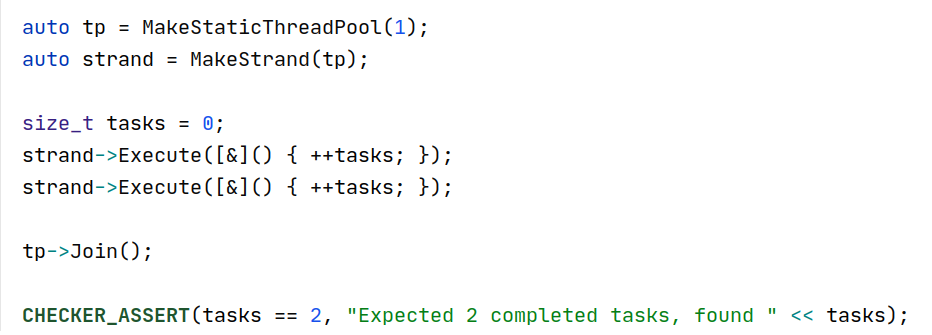
\includegraphics[scale=0.5]{strandtest}}
	}
	\bigskip
	\caption{Тест для Strand-а.}\label{fig:strandtest}
\end{figure}

\else

\begin{listing}
	\centering
	
	\begin{minted}{c++}
    
auto tp = MakeStaticThreadPool(1);
auto strand = MakeStrand(tp);

size_t tasks = 0;
strand->Execute([&]() { ++tasks; });
strand->Execute([&]() { ++tasks; });

tp->Join();

CHECKER_ASSERT(tasks == 2, "Expected 2 completed tasks, found " << tasks);

	\end{minted}
	\caption{Тест Strand-а.}
	\label{strandtest}
\end{listing}

\fi

Несмотря на простоту теста, за счет перебора всех исполнений model checker находит описанный выше race condition.
